
%%%%%%%%%%%%%%%%%%

\chapter{Introduction to Machine Learning}
\section{Machine Learning}
Machine learning in the context of econometrics is interested in model selection for prediction - finding the parsimonious model in the context of a very large dataset. It ranges from regularized models such as LASSO, Ridge regression, and elastic nets and methods that are much more involved - random forests and neural networks. All of them differ in how they fine-tune the model. \par
\section{Model Selection}
Often, we are interested in controlling a large set of covariates (e.g. propensity score). We can generalize this to the structure where structure refers to specification as well as parameter values. In determining the structure, we face a trade-off: We are tempted to increase the number of covariates since it allows us to fit the data better. However, in doing so, we risk overfitting - the out-sample prediction can perform poorly in terms of variance. Therefore, some method to penalize complexity is required. 
\par
We start with a set $\mathcal{M}$ of candidate models. Then for a model $M\in\mathcal{M}$, we define a penalty parameter $p(M)$ that increases in complexity. Two classical information criteria include
\begin{itemize}
\item Akaike's Information Criterion: Choose $M$ satisfying
\[
\max_{M}\left(\max_\theta \sum_{i=1}^n \log{l_i(\theta;M)}-p(M) \right)
\]
\item Bayesian Information Criterion: Choose $M$ satisfying
\[
\max_{M}\left(\max_\theta \sum_{i=1}^n \log{l_i(\theta;M)}-p(M)\frac{\log{n}}{2} \right)
\]
\end{itemize}
The subtle difference between the two is that BIC tends to be harsher for complexities. This can be seen since for $n>8$, the penalty term is larger. Moreover, the derivation of BIC is based on a Bayesian probabilistic framework - If a selection of candidate models includes a true model for the dataset, then the probability that BIC selects the correct model approaches to 1 as training sample size increases (From Hastie, Tibshirani, Friedman "The Element of Statistical Learning", 2016). Therefore, BIC performs better for selecting the model within the given sample. For out-sample performance, AIC performs better. Both of them, however, can be impractical to calculate when we work with large models. This can be common especially if we allow for multiple levels of interaction between the covariates. In other words, if $p$ is a number of potential covariates, and $n$ is the sample size, we run into the case where $p>>n$. \par
One way out is to penalize complexities with the convex norm penalties. Define
\[
\Vert \theta \Vert _m = \sqrt[m]{\sum_{k=1}^p \vert \theta_k \vert ^m}
\]
and for $m=0$, we have $\Vert \theta \Vert _p=p$, penalties for the two information criteria above. Depending on the selection of $m$, we get different estimators that incorporates different shrinkage mechanisms - Ridge for $m=2$ and LASSO for $m=1$. \par
The general idea of shrinkage is as follows: We know that OLS is BLUE - It has the least variance among the linear, unbiased estimators. But what if we are willing to relax the 'unbiased' condition? Then can we find some estimators that have lower variance and even a lower mean squared error? James, Stein (1961) shows that it is possible and generalizable. \par 
Ridge and LASSO builds upon this idea, but uses different regularization methods. Consider the setup $Y_i=X_i\theta_0+\epsilon_i$. Ridge regression minimizes
\[
\sum_{i=1}^n(Y_i-X_i\theta_0)^2+\lambda\sum_{k=1}^p \theta_k^2 \ \ \left(\sum_{k=1}^p \theta_k^2=\Vert \theta\Vert_2^2\right)
\]
and yields
\[
\hat{\theta} = (X'X+\lambda I_p)^{-1}X'y
\]
Note that as $\lambda$ increases, the $(X'X+\lambda I_p)^{-1}$ term decreases, which drives the coefficients close to 0 and reduce overfitting. With LASSO, the minimization is 
\[
\frac{1}{n}\sum_{i=1}^n(Y_i-X_i\theta_0)^2+\lambda\sum_{k=1}^p |\theta_k| 
\]
and the first order condition can be written as
\[
\frac{2}{n}\sum_i X_{ik}(y_i-X_i\theta)=\lambda s_k, \ \ s_k = \begin{cases}1 & (\hat{\theta}_k>0) \\ -1 & (\hat{\theta}_k<0)\\ [-1,1] & (\hat{\theta}_k=0)\end{cases}
\]
Where $\lambda s_k$ is not necessarily 0, consistent with the idea that we are open to allowing for some bias in order to find an estimator that reduces MSE. 
\par So what is the difference between LASSO and Ridge? Ridge regression drives your coefficients towards 0 but not equal to it. So when it comes to model selection in terms of ruling out irrelevant variables, LASSO does better. This idea is captured by the figure below. As far as computation is concerned, Ridge has a quicker computation speed and works relatively better with multicollinearity.  So the choice of the estimation method depends on your goal of minimizing MSE as well as computation power (but with modern computational power, LASSO is preferred to Ridge). 
\begin{figure}[H]
\centering
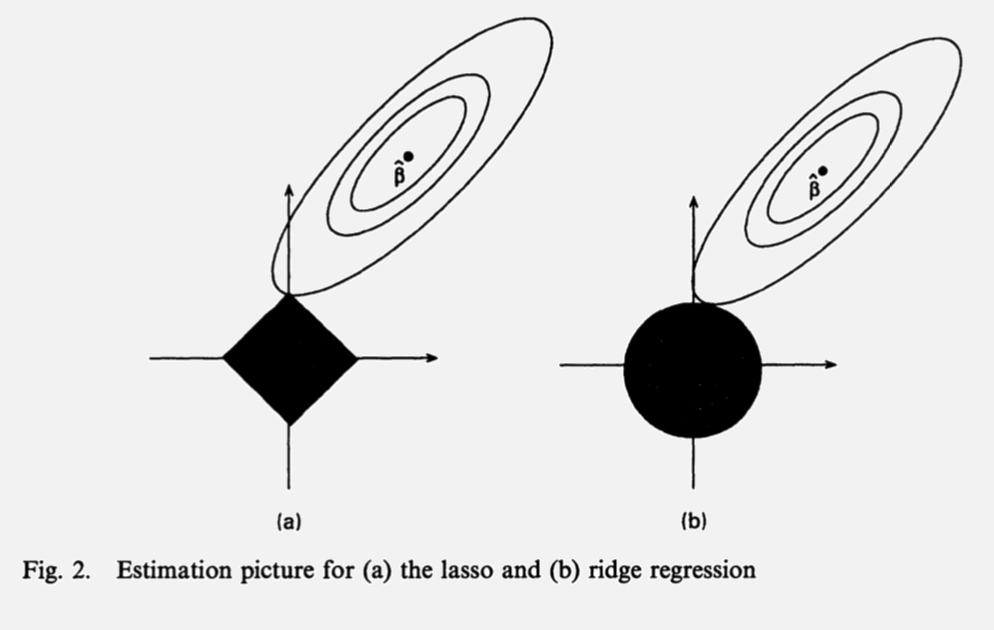
\includegraphics[width=0.67\textwidth, keepaspectratio]{lasso.png}
\caption{Ridge vs LASSO}
\end{figure}
\begin{mdframed}[backgroundcolor=yellow!5] 
\begin{comment}[Can you do both at once?] With \textbf{Elastic Net Regression}, you can. The idea is to use a penalty term that is a convex combination of both $l_1$ and $l_2$ penalty term. Specifically, 
\[
\sum_{i=1}^n(Y_i-X_i\theta_0)^2+\lambda\sum_{k=1}^n\left[\alpha \Vert \theta \Vert_1^2 +(1-\alpha)\Vert \theta \Vert_2^2\right]
\]
If $\lambda=0$ we have an OLS. For $\lambda\neq0$, if $\alpha=1$, we have LASSO, and if $\alpha=0$ we get Ridge. 
\end{comment}
\begin{comment}[Least Angle Regression (LARS)]
The algorithm is as follows
\begin{enumerate}
\item Start with a constant model: For all non-constant covariates, coefficients are 0 and $\lambda=\infty$. 
\item Then, find the covariate that has the largest covariance with the residual. 
\item Change the coefficient for that variable in the same direction as its covariance with the residual ($Y_i- \hat{Y}_i$) until you find a different covariate that has as much covariance with the residuals.  $\lambda$ decrease and $\theta$ is updated along the way.
\item Change the coefficient for the two variables until you find a third variable with the same covariance with the residual. 
\item Stop when all predictors are in the model
\end{enumerate}
When the covariate has the largest covariance with the residual, its angle is smallest. Hence the name LARS. The following figure captures how it works. 
\begin{figure}[H]
\centering
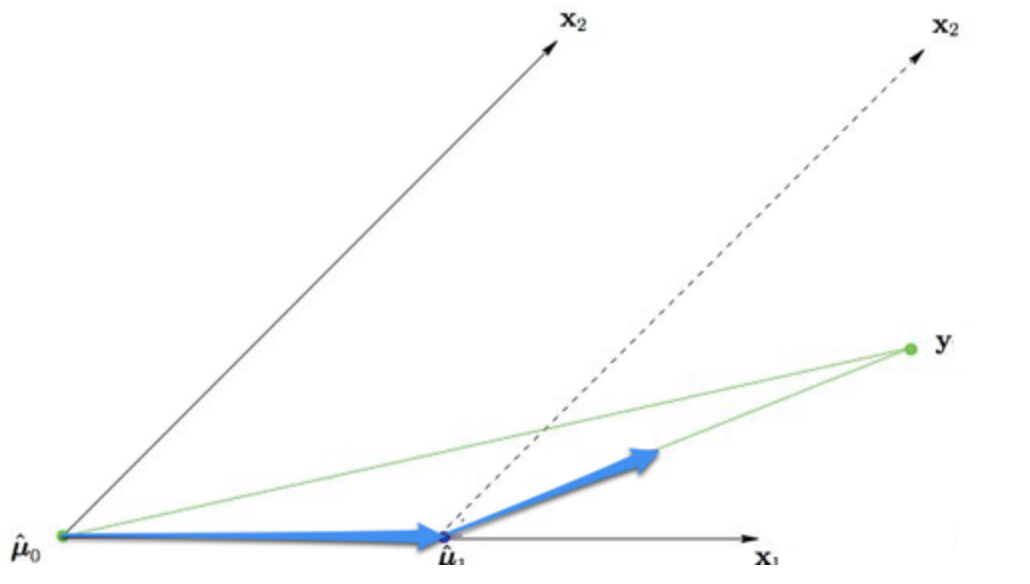
\includegraphics[width=0.67\textwidth, keepaspectratio]{lars.png}
\caption{LARS with two variables}
\end{figure}
\end{comment}
\end{mdframed}
So what is the optimal $\lambda$? It depends on your goal. If your goal is to minimize the prediction error, you can use the following cross-validation methods to come up with one
\begin{itemize}
\item Leave-one-out: Leave one observation out at a time
\item Training vs Test sample: You split the sample into two, build a model given some $\lambda$ and gain prediction error from the test sample. Then, select $\lambda$ minimizing the prediction error there.
\item $K$-fold cross validation:  For $K-1$ blocks, estimate the model given some $\lambda$ and compute the error on the remaining block. Get this for $K$ blocks and compute the average error. Select $\lambda$ minimizing the error. 
\end{itemize}
\section{Some Primer on the Consistency of LASSO}
We want to identify what the true model is in a setting with potentially an infinite number of covariates. To do that, we first set a sparsity assumption, where the number of nonzero coefficients is not too large. As a thought experiment, we increase the number of regressors as $n\to\infty$ in order to approximate the true model. To satisfy the assumption, we require that the number of nonzero regressors to rise at a slower rate than $n$. Specifically, $s_n = o\left(\sqrt{\frac{n}{\log p}}\right)$. \par
If we let $\lambda_n = O\left(\sqrt{\frac{\log p}{n}}\right)$ and have $s_n=o\left(\sqrt{\frac{n}{\log p}}\right)$, then we can show that the prediction error goes to 0 and the LASSO estimator is consistent. Or
\[
\frac{1}{n}\sum_i(X_i\hat{\theta}_n-X_i\hat{\theta}_{0n})^2=O_p(\lambda_n^2s_n)
\]
and 
\[
\Vert \hat{\theta}_n-\hat{\theta}_{0n}\Vert_1 = o_p(\lambda_n s_n) = o_p(1)
\]
This comes at the cost of a slightly slower rate of convergence, which is tolerable as long as it is faster than $n^{-1/4}$.


\section{Random Forests}
Random forests use a series of decision trees - a stack of two-way splits with several number of depths - to solve a classification problem. The splits are based on covariate $k$ being above or below a certain threshold. The process stops at some depth and predict with the mean of $y$ at the terminal node $x$ belongs to. The covariate and the threshold combination that determine the split are selected so as to have the largest separation possible. This is commonly referred to as a `greedy' way of creating random forests.  \par
The detailed way of constructing random forests are as follows. Randomness is injected in several levels: one to select a random sample to train each tree on. Second level of randomness is involved in selecting variable candidates to determine splits for the trees. At the end, we get a prediction for any $x$, average of the predictors of the trees. We can also estimate the prediction error at any observation $x_i$ and gain expected prediction error overall. We can also identify which covariates contributed the most the the prediction using the variance-importance plots. This is where the random forests gain the advantage of interpretability - explaining as to why the results of the prediction came out to be as it is (not just spitting out the number). \par
There are some trade-offs. We want some level of depths in order to reduce the variance in the prediction and get a better fitting. However, too much depth will lead to overfitting. It is usually very difficult to find the happy medium. \par
Below is the example of the decision brought from Varian (2014). A random forests would be obtained by multiple trees, each with different sample (selected through bootstrap) and different variable and threshold combination. 
\begin{figure}[H]
\centering
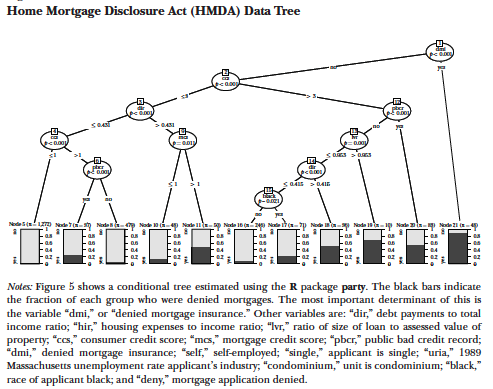
\includegraphics[width=0.7\textwidth, keepaspectratio]{randomforest.png}
\caption{From Varian (2014), Figure 5}
\end{figure}\par
\section{Double Machine Learning De-biasing Technics}
Often we are interested in testing for regarding the value of the parameter of interest. For instance, the average treatment effect under the conditional independence assumption. Specifically, we assume $(\epsilon_i(1),\epsilon_i(0))\perp\!\!\!\perp u_i|X_i$ where $X_i$ contains a large set of covariates. What we may do is to estimate the propensity score using machine learning techniques such as LASSO. Then, estimate the average treatment effect with the formula of our choice. Ideally, we want to conduct some standard tests. \par
Here is the problem - what we have for the propensity score is an estimate with some error. So depending on the size of this error, the estimate of the average treatment effect could be affected. Moreover, the propensity score is just a means towards our ultimate goal of obtaining the average treatment effect - it is merely a nuisance parameter. Since what we are doing involves errors at two different stages, we need a double machine learning de-biasing technics. Specifically, we decouple the propensity score and the treatment effect by applying Neyman Orthogonalization. In principle, what this method allows us to do is to do a two-step estimation by getting the estimate for the propensity score and then estimate the ATE without having to worry too much about the contaminated standard errors originating from the fact that we are not using the exact the propensity score. \par
In our case, what we can do is to
\begin{enumerate}
\item Split data into $K$ folds
\item Use LASSO to estimate $\hat{P}_k=\Pr(D_i=1|X_i)$ in all folds except the $k$th one. $k$ can be from 1 to $K$. 
\item If we are using inverse probability weighting method, for instance, we can get
\[
\widehat{ATE}=\sum_{k=1}^K\left[\frac{\sum_{i\in k}\frac{Y_iD_i}{\hat{P}_k(X_i)}}{\sum_{i\in k}\frac{D_i}{\hat{P}_k(X_i)}}-\frac{\sum_{i\in k}\frac{Y_i(1-D_i)}{1-\hat{P}_k(X_i)}}{\sum_{i\in k}\frac{(1-D_i)}{1-\hat{P}_k(X_i)}}\right]
\]
and use standard asymptotics to conduct tests. 
\end{enumerate}
